\documentclass[11pt]{book}
\usepackage[hidelinks]{hyperref}
\usepackage{float}
\usepackage{graphics}
\setcounter{tocdepth}{4}
\setcounter{secnumdepth}{3}
\title{Development of the International System}
\begin{document}
\maketitle
\tableofcontents
\part{Lecture Note.}
	\chapter{Week 1, Day 1.}
			\paragraph{04 August 2025; Kasira, Teewin, Pongphisoot.}
		\section{Introduction to the Course.}
			\subsection{Why Study the Development of the International System?}
				\begin{itemize}
					\item Rationale.
					\item What is an international system?
						\subitem Organisation of political authority in a large scale.
					\item Key questions on "The Order".
						\subitem Designed by whom? For whom? What can we do in given order?
						\subitem What about ethical consideration?
						\subitem History is your friend.
				\end{itemize}
				
				%%%%%%%%%
				
		\section{Empirical Theory of Knowledge.}
					\subsection{Empirical Theory of Knowledge: Positivist Approach.}
					Outside stimuli are separated from one's capacity to process them.
						\paragraph{Positivist:}
					Those who argue that facts point to an absolute conclusion.
							\begin{itemize}
								\item History could be studied as \textbf{hard science}.
								\item E.H Carr argues that this is \textbf{bias}.
										\begin{itemize}
											\item Positivists presuppose that history is like hard science:
												\begin{itemize}
													\item \textbf{Dependent} Variable = Conclusion.
													\item \textbf{Independent} Variable = Facts.
													\item \textbf{Controlled} Variable = Objectivity.
												\end{itemize}
										\end{itemize}
							\end{itemize}

					%%%%%%%%%%%%%%%%%%%%%%
					
					\subsection{Subjectivity in History.}
						\begin{itemize}
							\item Exploitation of Subjectivity.

								\begin{itemize}
									\item Can be taken advantage of by anymore, whether good or bad.
									\item Can be intentional or unintentional.
								\end{itemize}
								
							\item Nation States, and Origin Myths.

								\begin{itemize}
									\item Create origin myths to foster a shared identity.
									\item Unite disparate groups of people.

								\end{itemize}

							\item Demagogues and Historical Reshaping.

								\begin{itemize}
									\item Reshape history to serve their aims.
								\end{itemize}
							\item Revisionists, and political objectives.
								\begin{itemize}
									\item Make changes to prevailing history narratives.
									\item Serve political objectives.
								\end{itemize}
						\end{itemize}						
						
						
					\subsection{Perception, and Analysis of History: Linear/Progressive Thinking.}
						\begin{itemize}
							\item Dependence on Societal Changes, and Time.
								\subitem Our understanding of history is influenced by how we view societal changes.
								\subitem Time plays a crucial role in shaping our perception of historical events.
							\item Linear/Progressive Thinking.
								\subitem Society is seen as moving forward or declining in a linear fashion.
								\subitem Many social evolution theories fall under this category.
								\subitem Example: Marxist Framework.
						\end{itemize}

				\subsubsection{Perception, and Analysis of History: Ripples of Effects.}
					\begin{itemize}
						\item Non-directional, and Non-linear Changes.
							\subitem Changes can recur, and induced by different factors.
						\item Absence of a Starting Point.
							\subitem Phenomena doesn't always have a clear origin,
						\item Simultaneous Occurrence.
							\subitem Many phenomena can happen together.
					\end{itemize}

				\subsubsection{Perspectives, and Arguments.}
					\begin{itemize}
						\item Importance of Perspectives.
							\subitem No correct or ultimate answers.
							\subitem Argument should be weighted with evidence.
							\subitem Balance heritage, and intellectual history.
							\subitem Economic Measurement.
					\end{itemize}


		\section{Eurocentrism.}
		\section{Transition, and Transformation 250-900CE.}
			\subsection{Introduction.}
				\subsubsection{Social Science Tradition.}
					\begin{itemize}
						\item Social Science Tradition Stemming from History.
						\item Ferdinand Braudel's World System Theory.
						\item Marxist, and Neo-Marxist Theory
						\item Social Evolution.
					\end{itemize}


				\subsubsection{Eurocentric Perspectives.}
					Highlight European (and North Atlantic) superiority in arguments surrounding convergence, and divergence of society.
				
				\subsubsection{Types of Eurocentrism.}

						\section{Ancient To Modern.}
			\subsection{The Axial Age.}
			\subsection{Expansionism, and Pastoralism.}
			\subsection{Rome.}
			\subsection{China.}
				\subsubsection{Sino-Sphere System.}
				
				
				\subsubsection{The Han Dynasty, and its Characteristics.}
					\paragraph{Centralized Government.}
						The Han Dynasty had a centralised government headed by an emperor who held absolute power. This allowed for effective decision-making, and implementation of policies.
					\paragraph{Civil Service System.}
						The Han Dynasty had a sophisticated civil service system based on meritocracy. Candidates were selected through rigorous examinations, and trained to become officials, ensuring a highly competent bureaucracy.
					\paragraph{Stability, and Well-being.}
						The institutions of the Han Dynasty, including its centralised government, and civil service system, allowed for stability, and promoted the well-being of their people.
					\paragraph{Well-Field System.}
						Equal field system was invented in 384CE:
						\begin{itemize}
							\item China operates, and equal land field system.
						\end{itemize}
			
				\subsubsection{The Rise of Imperial China.}
					Establishment of a cultural community, de facto independent states in competition of each other.
					\begin{itemize}
						\item Zhou kings (771BCE-256BCE) kept losing power to overlords.
						\item Spring, and Autumn Period would be the beginning to an end of decentralised Chinese governance.
					\end{itemize}
					
					
				\subsubsection{Core Chinese State Characteristics.}

%					\begin{figure}[H]
% 					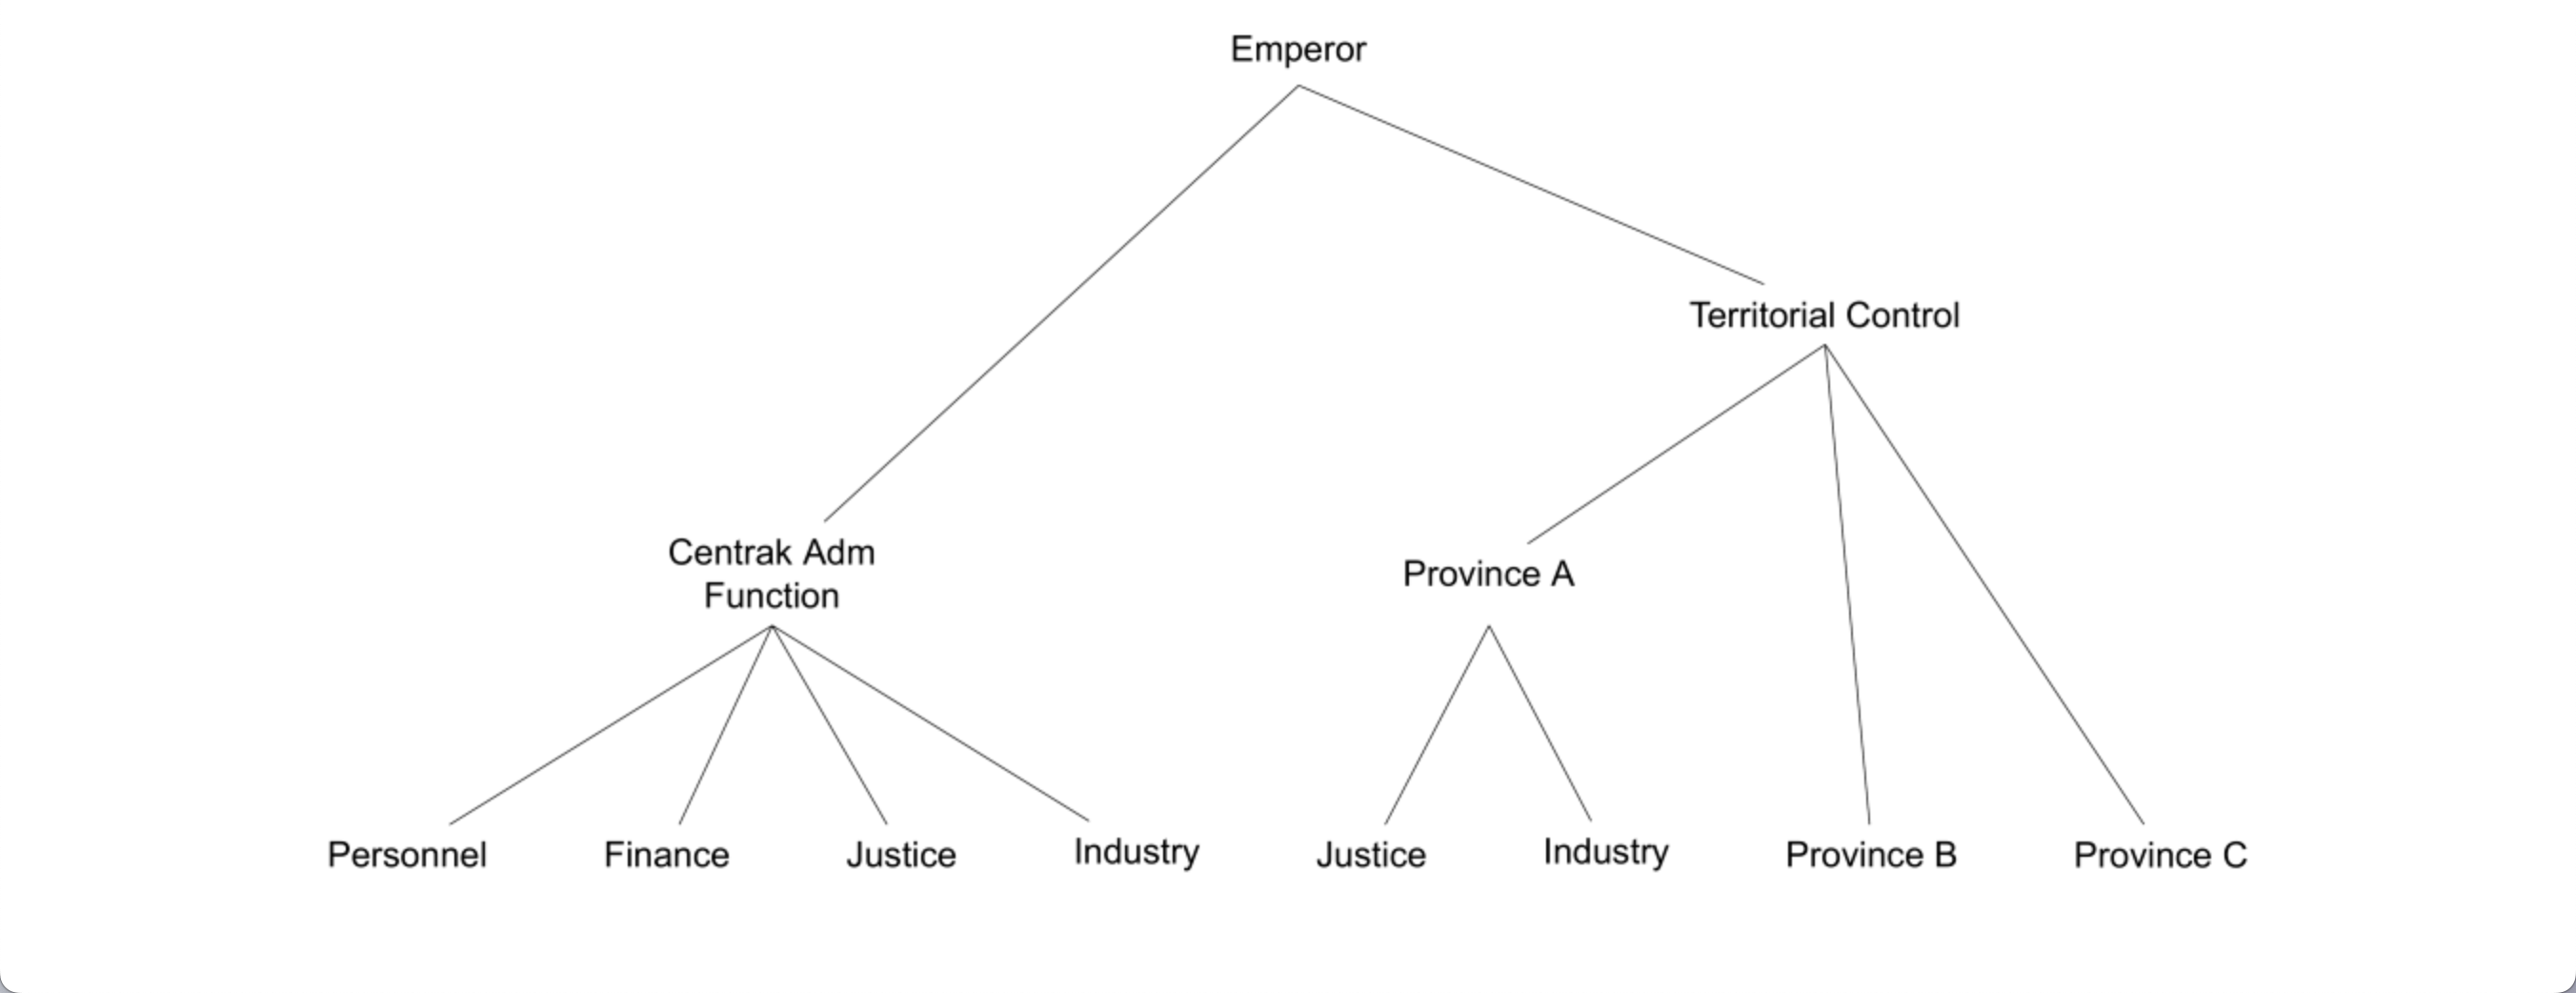
\includegraphics{Photos/Chinese Hierachy.png}
%						 \caption{Hierachy.}
%					\end{figure}

				\subsubsection{Civil Service System.}
					\paragraph{Merit-Based System.}
				
			\subsection{Indian.}
				\subsubsection{Pastorialism.}
				


		\section{Book: A History of Europe from 400 to 1000.}
			\href{Books/Empires In World History PDF.pdf}{Book.}

		\section{Book: Empires in World History: Power, and the Politics of Differences.}
			
			\subsection{The Rise of Early Empires, and Their Foundations.}
				Empires have been a significant, and influential force throughout world history, shaping the political, economic, and social landscapes of entire regions.
				
				The concept of an empire generally refers to: a large political unit, often comprising multiple territories and diverse populations, governed by a central authority.

				\textbf{Empires differ from other forms of political organization in their expansive nature and the integration of distinct cultures under a singular rule.}

				The characteristics defining empires include:
				\begin{itemize}
					\item  Vast territorial expanse.
					\item  Centralized administrative control.
					\item  The incorporation of various ethnic and cultural groups.
				\end{itemize}

				Empires exhibit a dual approach to governance-combining coercion through military might and persuasion via administrative strategies and cultural assimilation. These attributes allow empires to exert control over extensive regions, often maintaining dominance over distant territories for prolonged periods.
			
			\subsection{Empire-Building Through Military Conquest and Diplomacy.}
			
				
		\section{Book: Eight Eurocentric Historian.}

		\section{Book: Civilisation Recast.}


\chapter{Week 2, Day 1.}

\chapter{Week 3, Day 1.}
	\section{Renaissance.}
\part{Course Summary.}
	\chapter{Topic}

\end{document}
